\documentclass[11pt]{article}

\input{./preamble.tex}

%%
%% DOCUMENT START
%%

\begin{document}


\newcommand{\widesim}[2][1.5]{
  \mathrel{\overset{#2}{\scalebox{#1}[1]{$\sim$}}}
}

\pagestyle{fancyplain}
\lhead{}
\chead{}
\rhead{}
\lfoot{\hrule UQ: Homework 3}
\cfoot{\hrule \thepage}
\rfoot{\hrule Ryan Skinner}

\noindent
{\Large Homework 2}
\hfill
{\large Ryan Skinner}
\\[0.5ex]
{\large ASEN 6519: Uncertainty Quantification}
\hfill
{\large Due 2016/03/29}\\
\hrule
\vspace{6pt}

%%%%%%%%%%%%%%%%%%%%%%%%%%%%%%%%%%%%%%%%%%%%%%%%%
%%%%%%%%%%%%%%%%%%%%%%%%%%%%%%%%%%%%%%%%%%%%%%%%%
\section*{Problem 1} %%%%%%%%%%%%%%%%%%%%%%%%%%%%
%%%%%%%%%%%%%%%%%%%%%%%%%%%%%%%%%%%%%%%%%%%%%%%%%
%%%%%%%%%%%%%%%%%%%%%%%%%%%%%%%%%%%%%%%%%%%%%%%%%

Use the Smolyak formula
\begin{equation}
\mathc{A}(q,d) = \sum_{q-d+1 \le |\mb{l}| \le q} (-1)^{q-|\mb{l}|} \; \binom{d-1}{q-|\mb{l}|} \; \left( I^{(l_1)} \otimes \cdots \otimes I^{(l_d)} \right)
\label{eq:smolyak}
\end{equation}
to identify and plot the tensor-product of $d=1$ Clenshaw-Curtis (CC) Smolyak sparse grids from which the example grid $\mathc{A}(q=4,d=2)$ in the problem statement is constructed. Comment on the polynomial accuracy of the $d=2$ grid, referencing appropriate literature as needed.

\subsection*{Solution}

With $q=4$ and $d=2$, the bounds of the sum in \eqref{eq:smolyak} are $3 \le |\mb{l}| \le 4$. This admits only the following values of $\mb{l} = \{ l_1, l_2 \}$:
\begin{align*}
|\mb{l}| = 3: &\qquad \{ 0,3 \} \qquad \{ 1,2 \} \qquad \hphantom{\{ 2,2 \}} \qquad \{ 2,1 \} \qquad \{ 3,0 \} \\
|\mb{l}| = 4: &\qquad \{ 0,4 \} \qquad \{ 1,3 \} \qquad \{ 2,2 \} \qquad \{ 3,1 \} \qquad \{ 4,0 \}
\end{align*}
Abscissas of the 1-D CC grids are computed with \lstinline|spquad|, and the tensor products resulting in the constituent 2-D grids are plotted in \figref{fig:prob1}.

\begin{figure}[h]
\centering
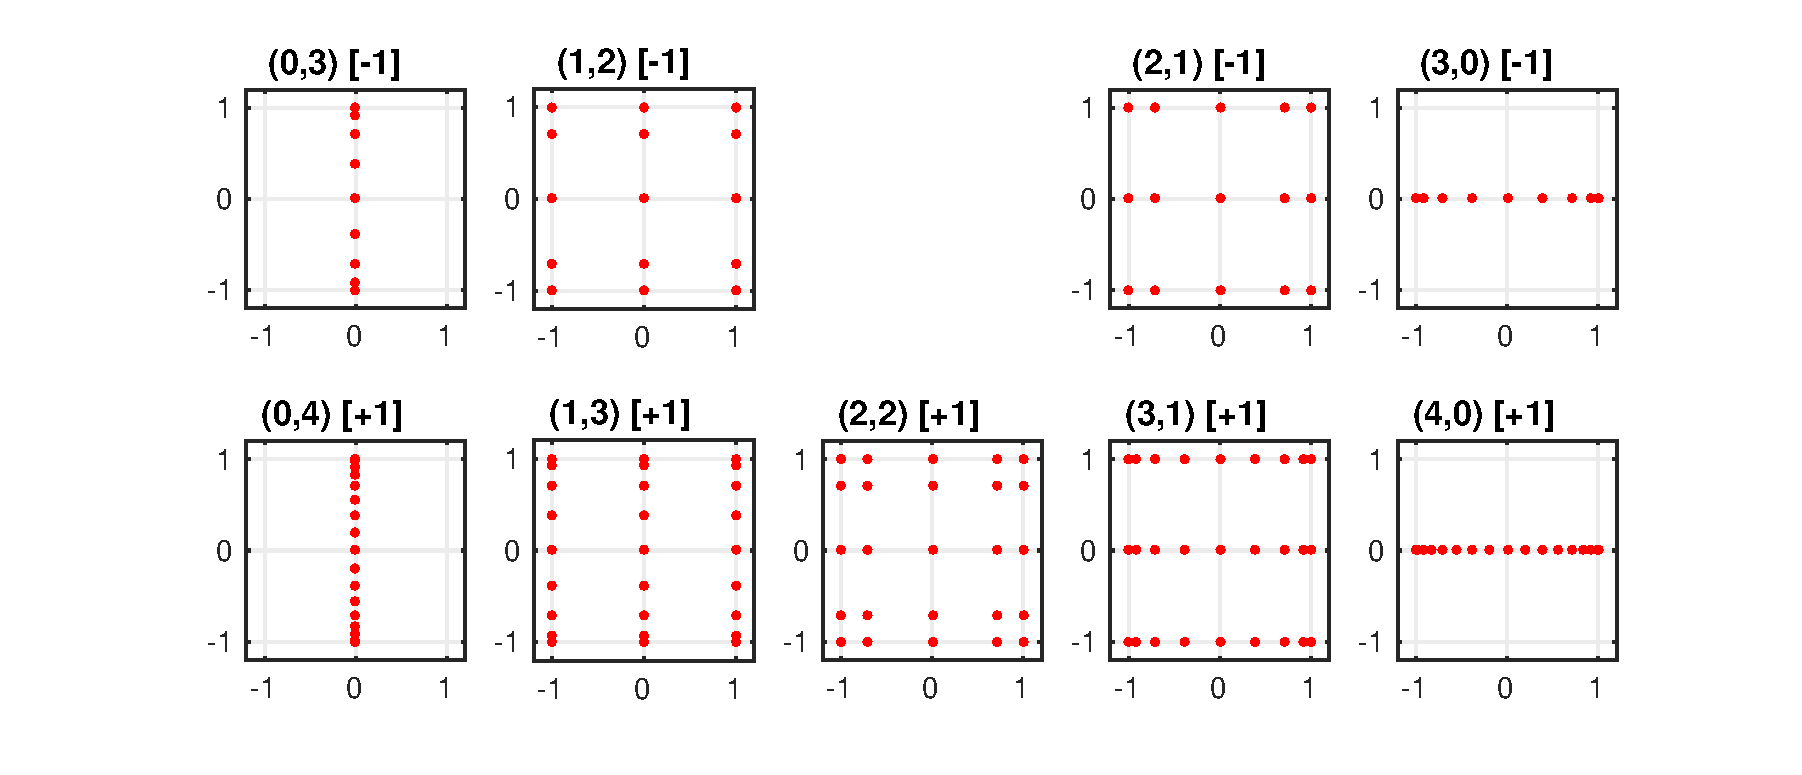
\includegraphics[width=0.9\textwidth, trim={1cm 0 1cm 0}]{prob1.eps}
\caption{Constituent grids that make up $\mathc{A}(4,2)$. Titles of sub-plots contain levels $l_1$ and $l_2$ in parentheses, and the value of $(-1)^{q-|\mb{l}|}$ in square brackets.}
\label{fig:prob1}
\end{figure}



%%%%%%%%%%%%%%%%%%%%%%%%%%%%%%%%%%%%%%%%%%%%%%%%%
%%%%%%%%%%%%%%%%%%%%%%%%%%%%%%%%%%%%%%%%%%%%%%%%%
\section*{Problem 2} %%%%%%%%%%%%%%%%%%%%%%%%%%%%
%%%%%%%%%%%%%%%%%%%%%%%%%%%%%%%%%%%%%%%%%%%%%%%%%
%%%%%%%%%%%%%%%%%%%%%%%%%%%%%%%%%%%%%%%%%%%%%%%%%

The thermal coefficient $K$ of a 1-D slab is defined on $\mathc{D} = (0,1)$ and is characterized by
\begin{equation}
K(x,\omega) = \overline{K} + \sigma \sum_{i=1}^d \sqrt{\lambda_i} \phi_i(x) y_i(\omega)
\end{equation}
where $\overline{K}=1$, $\sigma=0.1$, and $\{ \lambda_i, \phi_i(x) \}_{i=1}^d$ are eigen-pairs of the covariance kernel
\begin{equation}
C_{KK}(x_1,x_2) = \exp \left( \frac{- | x_1-x_2 | }{\ell} \right), \qquad (x1,x2) \in \mathc{D} \times \mathc{D}
\end{equation}

Moreover, $\{y_i\}$ are i.i.d. $U(-1,1)$. We would like to compute the statistics of the temperature field by solving the governing steady-state stochastic heat equation
\begin{equation}
\begin{aligned}
\pp{}{x} \left( K(x,\omega) \pp{u(x,\omega)}{x} \right) &= 1.0, \qquad x \in \mathc{D}, \\
u(0,\omega) &= 0, \\
u(1,\omega) &= 0,
\end{aligned}
\label{eq:pde}
\end{equation}

Setting $\ell = 2.0$, use the Homework \#1 code to compute the eigen-pairs $\{ \lambda_i, \phi_i(x) \}_{i=1}^d$ with $d=2$.

\begin{enumerate}

\item Compute $\xpect{u(x)}$ and $\var(u(x))$ of $u(x,\omega)$ using Latin Hypercube Sampling (LHS), with samples generated using your own code. Verify convergence of the mean and variance as you draw more samples.

\item Compute the same mean and variance using stochastic collocation with a tensor-product grid of the Clenshaw-Curtis rule. You can use the Matlab function \lstinline|spquad.m|, available on our course webpage, to obtain the abscissas and weights of the CC quadrature rule in dimension $d=1$. To obtain a reference solution for these comparisons, use $N=33$ quadrature points along each direction to compute the solution mean and variance. Verify convergence by increasing the number of quadrature points at $N = 1, 4, 16, 32$.

\item Compute the mean and variance using stochastic collocation of a Smolyak sparse grid with CC abscissas. Verify convergence in the manner discussed above.

\item On a single plot, compare the convergence of the estimates of the mean at $x=0.5$ based on standard Monte Carlo sampling, Latin Hypercube Sampling, tensor-product grid stochastic collocation (CC rule), and Smolyak sparse grid stochastic collocation (CC rule) as a function of the number of samples. Verify that the convergence rate of standard MC is $1/\sqrt{N}$. Repeat this comparison for the estimate of the variance at $x=0.5$.

\item Comment on the growth of the number of Smolyak abscissas and the feasibility of doing stochastic collocation when the correlation length is $\ell = 0.1$.

\end{enumerate}


%\vspace{2in}
%\begin{table}[h]
%\centering
%\begin{tabular}{ll}
%\toprule
%Quantity & Value \\
%\midrule
%$\xpect{u_\tmax}$ & 0.12568 \\
%$\var(u_\tmax)$ & 0.03379 \\
%$P(\cdot)$ & 1.59 \% \\
%\bottomrule
%\end{tabular}
%\vspace{1em}
%\caption{Relevant quantities in \eqref{eq:probability} computed from 250,000 realizations using 1,001 grid points.}
%\label{tbl:probabilities}
%\end{table}

%%
%% DOCUMENT END
%%
\end{document}
